\section{Metodologia}
\label{sec:metodologia}

Esta seção descreve os procedimentos adotados na implementação do conversor
VR-BESS e de seus subsistemas (painel fotovoltaico e banco de baterias) em
ambiente MATLAB/Simulink, com os componentes elétricos representados no
domínio físico do Simscape Electrical.

\subsection{Topologia do Conversor Implementada}
\label{subsec:topologia_impl}

A topologia VR-BESS implementada segue a estrutura descrita por
\cite{srinivasa2016vrbess}, composta por dois indutores ($L_s$, $L_{bat}$),
duas chaves semicondutoras ($S_1$, $S_2$) e três diodos ($D_1$, $D_2$,
$D_3$), conforme ilustrado na Fig.~\ref{fig:topologia}. O nó de comutação da
porta fotovoltaica é formado por $L_s$, $S_1$ e $D_3$ (caminho de regulação
de tensão para a carga) e $D_2$ (caminho de carregamento da bateria); o nó
de comutação da porta de armazenamento é formado por $L_{bat}$, $S_2$ e
$D_1$ (caminho de descarga da bateria para o barramento de saída).

Na proposta original de \cite{srinivasa2016vrbess}, $S_1$ e $S_2$ operam de
forma sincronizada sob um único sinal PWM. Neste trabalho, as duas chaves
são tratadas como variáveis de controle \emph{independentes} dentro do
conjunto finito de estados do FCS-MPC, resultando em quatro estados de
comutação candidatos ($S_1,S_2 \in \{0,1\}^2$) a cada período de
amostragem, em vez dos dois estados da modulação síncrona original. Essa
adaptação é o que torna pertinente a aplicação do FCS-MPC -- discutido na
Seção~\ref{subsec:fcsmpc} -- a essa topologia, permitindo o controle
desacoplado da tensão de saída e da corrente de bateria.

\subsection{Derivação da Razão Cíclica}
\label{subsec:duty_cycle}

As razões cíclicas aplicadas às chaves $S_1$ e $S_2$ são obtidas a partir
do equacionamento por balanço volt-segundo nos indutores $L_s$ e $L_{bat}$,
apresentado por \cite{kai2024projeto} para o conversor VR-BESS. Para o
Modo~1 de operação (regulação de tensão com carregamento simultâneo da
bateria), as razões cíclicas de $S_2$ e $S_1$ são dadas, respectivamente,
por

\begin{equation}
D_i = 1-\frac{V_s}{V_o}, \qquad D_{ii} = D_i+\frac{V_{bat}}{V_o}.
\label{eq:duty_modo1}
\end{equation}

Diferentemente da tensão de bateria $V_{bat}$, cujo valor em regime é bem
aproximado pela tensão de circuito aberto do banco série-paralelo adotado
($V_{bat}\approx N_{s,bat}\times E_0$), a tensão do painel fotovoltaico
$V_s$ não é determinada apenas pela associação série/paralelo
($N_{s,mod}$, $N_{p,mod}$): por se tratar de uma fonte de corrente não
ideal (Eq.~\eqref{eq:pvmodel}), seu valor em regime depende também da
corrente demandada pelo conversor, que por sua vez depende da própria
razão cíclica e da corrente de carregamento da bateria $I_{bat}$. Assim,
$V_s$ deve corresponder ao ponto de operação autoconsistente do arranjo
sob a corrente efetivamente demandada no Modo~1 -- e não à tensão de
máxima potência nominal do arranjo
($V_{MP}=N_{s,mod}\times V_{MP,1}$), que só corresponderia ao ponto de
operação real caso a corrente demandada coincidisse exatamente com a
corrente de máxima potência do arranjo ($I_{mpp}=N_{p,mod}\times I_{MP,1}$).

Esse ponto de operação é obtido resolvendo-se, de forma autoconsistente,
o sistema formado pela Eq.~\eqref{eq:duty_modo1}, pela equação de corrente
do Modo~1,

\begin{equation}
I_s = \frac{V_{bat}/V_o}{1-D_i}\,I_{bat} + \frac{1}{1-D_i}\,I_o,
\label{eq:is_modo1}
\end{equation}

e pelo modelo de diodo único do painel (Eq.~\eqref{eq:pvmodel}), uma vez
que $D_i$ depende de $V_s$ (Eq.~\eqref{eq:duty_modo1}), $I_s$ depende de
$D_i$ (Eq.~\eqref{eq:is_modo1}), e $V_s$ é por sua vez determinado por
$I_s$ através da curva $I$-$V$ do arranjo. Resolvendo numericamente esse
sistema por iteração de ponto fixo para $V_o=400$~V, $R_o=160\,\Omega$
($I_o=2{,}5$~A), $V_{bat}=252$~V ($N_{s,bat}=15$) e a corrente de
carregamento observada $I_{bat}\approx1{,}47$~A, com o arranjo
fotovoltaico configurado em $N_{s,mod}=17$, $N_{p,mod}=2$, obtém-se o
ponto de operação autoconsistente $V_s\approx344{,}90$~V,
$I_s\approx3{,}973$~A, e as razões cíclicas correspondentes:

\begin{equation}
D_i = 13{,}77\%\ (S_2), \qquad D_{ii} = 76{,}77\%\ (S_1).
\label{eq:duty_valores}
\end{equation}

\begin{figure}[h]
\centering
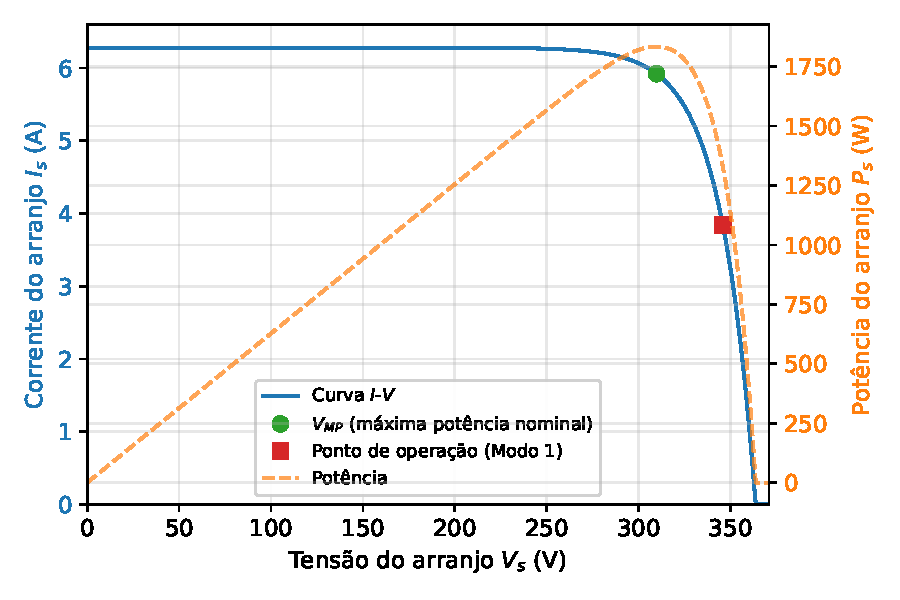
\includegraphics[width=\linewidth]{Figuras/curva_iv_pv.pdf}
\caption{Curva $I$-$V$ e de potência do arranjo fotovoltaico
($N_{s,mod}=17$, $N_{p,mod}=2$), com a tensão de máxima potência nominal
($V_{MP}$) e o ponto de operação autoconsistente do Modo~1 destacados.}
\label{fig:curva_iv_pv}
\end{figure}

\begin{figure}[h]
\centering
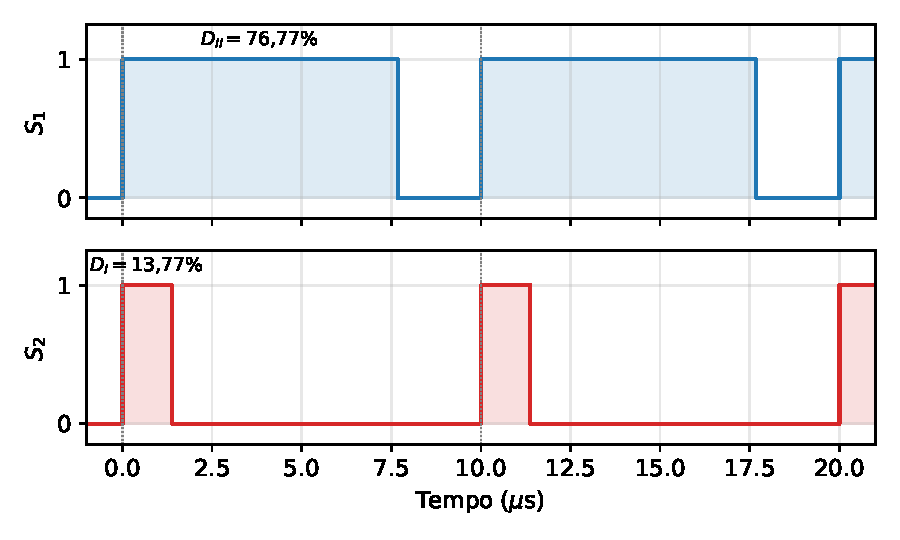
\includegraphics[width=\linewidth]{Figuras/pwm_pulsos.pdf}
\caption{Sinais de comutação de $S_1$ e $S_2$ dentro de um período de
comutação $T_{sw}=10\,\mu\text{s}$, com $S_2$ (duração $D_i$) contido no
intervalo de fechamento de $S_1$ (duração $D_{ii}$), ambos iniciando em
$t=0$.}
\label{fig:pwm_pulsos}
\end{figure}

\subsection{Modelagem do Painel Fotovoltaico}
\label{subsec:modelagem_pv_impl}

O painel fotovoltaico foi implementado como um subsistema mascarado
combinando um bloco \texttt{MATLAB Function} -- que resolve o modelo de
diodo único apresentado na Eq.~\eqref{eq:pvmodel} -- com os componentes
físicos do Simscape responsáveis pela interface elétrica: um sensor de
tensão, que mede $V$ nos terminais do painel e o converte para o domínio de
sinal (\texttt{PS-Simulink Converter}); e uma fonte de corrente controlada
(\texttt{Controlled Current Source}), que injeta a corrente calculada $I$
de volta ao circuito físico após a conversão inversa
(\texttt{Simulink-PS Converter}). Essa arquitetura fecha a malha algébrica
$V \rightarrow I \rightarrow V$ inteiramente no domínio físico do Simscape,
sem necessidade de tratamento explícito de laço algébrico no domínio de
sinal.

Os parâmetros de catálogo adotados correspondem ao painel monocristalino de
\cite{ayaz2014improved} ($I_{SC,ref}=3{,}14$~A, $V_{OC,ref}=21{,}4$~V,
$N_s=36$ células), complementados por coeficientes de temperatura típicos
de painéis dessa classe ($K_v=-0{,}080$~V/°C, $K_i=0{,}0024$~A/°C), uma vez
que esses coeficientes não constam no artigo de referência. As entradas de
irradiância ($G$) e temperatura ($T$) são fornecidas por blocos
\texttt{Stair Generator}, permitindo a aplicação de degraus que emulam
variações de nebulosidade e temperatura ambiente durante a simulação. O
bloco mascarado permite ainda configurar a associação série/paralelo do
arranjo, por meio dos parâmetros $N_{s,mod}$ (módulos em série) e
$N_{p,mod}$ (fileiras em paralelo), escalando a tensão de circuito aberto e
a corrente de curto-circuito equivalentes do arranjo, respectivamente.

\subsection{Modelagem da Bateria}
\label{subsec:modelagem_bat_impl}

O banco de baterias foi modelado segundo o modelo dinâmico genérico de
Shepherd, na formulação proposta por \cite{tremblay2007generic}, amplamente
utilizado em simulações de sistemas híbridos e veiculares. A tensão de
circuito aberto é dada por

\begin{equation}
E = E_0 - K\frac{Q}{Q - it}\,it + A\,e^{-B\cdot it},
\label{eq:battery_ocv}
\end{equation}

em que $E_0$ é a tensão constante do modelo, $K$ a constante de
polarização, $Q$ a capacidade nominal, $A$ e $B$ os parâmetros da zona
exponencial da curva de descarga, e $it$ a carga já extraída da bateria
(Ah). A tensão nos terminais é então

\begin{equation}
V_{bat} = E - R\,I_{bat},
\label{eq:battery_terminal}
\end{equation}

onde $R$ é a resistência interna e $I_{bat}$ a corrente da bateria
(convenção positiva para descarga). A variável $it$ não é calculada
internamente ao bloco \texttt{MATLAB Function}, por se tratar de uma
grandeza dinâmica: ela é obtida por um bloco \texttt{Integrator} externo,
que integra $I_{bat}/3600$ ao longo do tempo, com condição inicial
$it_0 = Q\,(1 - SOC_0/100)$ correspondente ao estado de carga inicial
desejado. O estado de carga percentual é obtido por
$SOC = 100\,(1 - it/Q)$.

A corrente de bateria $I_{bat}$ é limitada por um resistor série cujo valor
cresce proporcionalmente ao excesso de corrente em relação a um limiar de
referência -- distinto para carga ($0{,}5\text{C}$, $1{,}15$~A) e descarga
($2\text{C}$, $4{,}6$~A) --, de modo que a corrente de regime pode assentar
acima do limiar nominal quando há potência excedente disponível no
arranjo fotovoltaico, sem que ocorra um corte abrupto de corrente.

De forma análoga ao painel fotovoltaico, a interface elétrica do subsistema
da bateria é composta por um sensor de corrente (medindo $I_{bat}$ em
série com o ramo) e uma fonte de tensão controlada
(\texttt{Controlled Voltage Source}), que aplica $V_{bat}$ calculado pela
Eq.~\eqref{eq:battery_terminal} de volta ao circuito físico.

Os parâmetros adotados para uma célula/módulo unitário
($E_0=16{,}8$~V, $K=0{,}0076$~V/Ah, $Q=2{,}3$~Ah, $A=0{,}26422$~V,
$B=26{,}5487$~Ah$^{-1}$, $R=0{,}01\,\Omega$) representam um banco de
baterias de íon-lítio genérico, com tensão nominal compatível com a tensão
de bateria considerada em \cite{srinivasa2016vrbess} ($V_{bat}\approx16$~V).
Assim como no painel fotovoltaico, o bloco mascarado do banco de baterias
permite configurar a associação série/paralelo do arranjo por meio dos
parâmetros $N_{s,bat}$ (módulos em série) e $N_{p,bat}$ (ramos em
paralelo), além do estado de carga inicial $SOC_0$.

\subsection{Implementação no Simulink/Simscape}
\label{subsec:implementacao}

Ambos os subsistemas (painel e bateria) seguem o mesmo padrão de
arquitetura: um bloco \texttt{MATLAB Function}, restrito ao domínio de
sinal do Simulink, é acoplado ao domínio físico do Simscape por meio de um
par de conversores (\texttt{PS-Simulink Converter} e
\texttt{Simulink-PS Converter}) e de um componente de medição e um de
atuação física correspondentes -- sensor de tensão e fonte de corrente
controlada no caso do painel; sensor de corrente e fonte de tensão
controlada no caso da bateria. Essa solução foi adotada em substituição aos
blocos pré-construídos de biblioteca (\texttt{PV Array} e \texttt{Battery}
do Simscape Electrical), não disponíveis no ambiente MATLAB Online
utilizado neste trabalho.

Nesta etapa de desenvolvimento, os parâmetros de catálogo de cada
subsistema foram inseridos diretamente no corpo das funções
\texttt{MATLAB Function}, com as entradas dos blocos restritas às
variáveis que efetivamente variam ao longo da simulação -- irradiância
($G$) e temperatura ($T$) no caso do painel, e corrente de bateria
($I_{bat}$) no caso do banco de baterias --, mantendo os demais parâmetros
de catálogo fixos internamente a cada função.

\subsection{Validação em Malha Aberta}
\label{subsec:validacao_ma}

Antes da síntese do controlador FCS-MPC, o conversor VR-BESS e seus
subsistemas de painel fotovoltaico e banco de baterias foram integrados e
validados em malha aberta, com o objetivo de verificar a correta
integração entre os blocos mascarados próprios (Seções~\ref{subsec:modelagem_pv_impl}
e~\ref{subsec:modelagem_bat_impl}) e o domínio físico do Simscape antes da
introdução da malha de controle.

\begin{figure}[h]
\centering
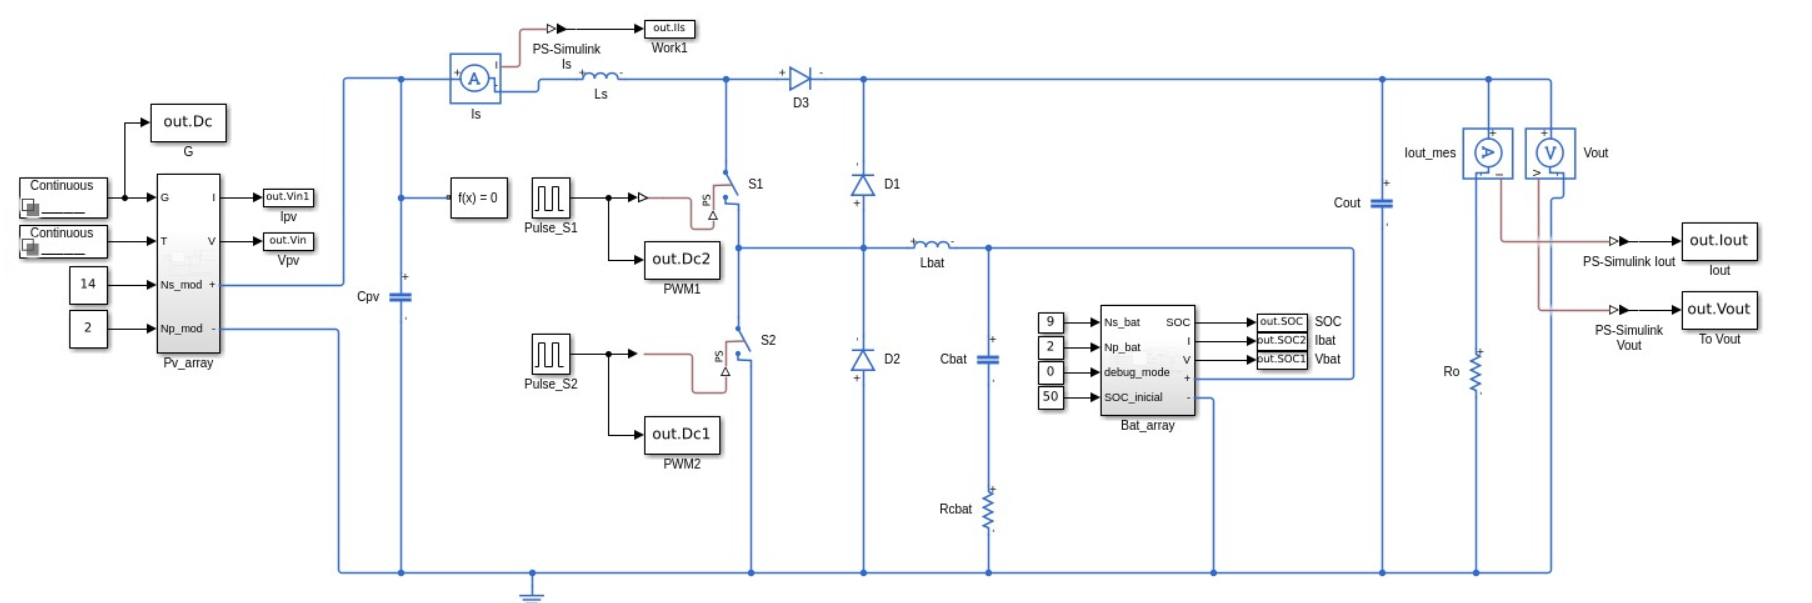
\includegraphics[width=\linewidth]{Figuras/vrbess_simulink_implementado.png}
\caption{Diagrama do modelo VR-BESS implementado no Simulink/Simscape
Electrical, incluindo os subsistemas mascarados de painel fotovoltaico
(\texttt{Pv\_array}) e banco de baterias (\texttt{Bat\_array}) e os
geradores de pulso (\texttt{Pulse\_S1}, \texttt{Pulse\_S2}) utilizados na
validação em malha aberta.}
\label{fig:simulink_implementado}
\end{figure}

Nessa configuração, as chaves $S_1$ e $S_2$ foram acionadas por geradores
de pulso independentes, com razão cíclica fixa dada pela
Eq.~\eqref{eq:duty_valores} e comutação em $f_{sw}=1/T_{sw}=100$~kHz
($T_{sw}=10\,\mu\text{s}$): $S_2$ com razão cíclica de $13{,}77\%$
($1{,}38\,\mu\text{s}$) e $S_1$ com razão cíclica de $76{,}77\%$
($7{,}68\,\mu\text{s}$), ambas com defasagem nula em relação ao início do
período de comutação. O painel fotovoltaico foi configurado com
$N_{s,mod}=17$ módulos em série e $N_{p,mod}=2$ fileiras em paralelo, sob
condição padrão de teste constante ($G=1000\,\text{W/m}^2$,
$T=25\,^{\circ}\text{C}$). O banco de baterias foi configurado com
$N_{s,bat}=15$ módulos em série e $N_{p,bat}=1$ ramo, partindo de um
estado de carga inicial $SOC_0=50\%$, com corrente de carregamento
limitada a $0{,}5\text{C}$ ($1{,}15$~A) e de descarga a $2\text{C}$
($4{,}6$~A). A carga foi fixada em $R_o=160\,\Omega$. Devido à largura
reduzida do pulso de $S_2$ frente ao passo de um solver de passo variável
padrão, adotou-se o \textit{Local Solver} do Simscape (Backward Euler,
passo fixo de $200$~ns) na rede física do conversor. A simulação foi
conduzida por $60$~ms, com as grandezas do domínio físico (tensões e
correntes medidas por sensor) registradas a $T_s=200$~ns. Os resultados
dessa validação são apresentados na Seção~\ref{sec:resultados}.
